\documentclass[main.tex]{subfiles}
\section{Component Overview}

\subsection{Project Overview}
In this subsection follows a description about the structure of the scripts.
The main script is called \textit{ReadLicensePlate.m} and can be found in listing~\vref{ReadLicensePlate}. 
In this script are a few things defined: 
\begin{itemize}
    \item The name of the input file.
    \item The amount of characters in a license plate.
    \item The amount of letters in a license plate.
\end{itemize}
The three different parts of this project are really visible in this script.
The first part: Image Manipulation is done in a different script but started from \textit{ReadLicensePlate.m}.
The second part: The search, also started in \textit{ReadLicensePlate.m}, is also mostly done in other scripts.
The last part: evaluation is done outside this script. 
The Image manipulation script can be found in listing~\vref{imageManipulation}.
This script uses only one custom made function, defined in listing~\vref{greyscale}.
Part two starts with calling the function findIndices, the script with the Matlab code can be found in listing~\vref{findIndices}.
The \textit{findIndices.m} function returns a possible license plate, to get to this license plate the function makes use of an other Matlab function called \textit{eliminateOptions.m}.
The code corresponding to this function can be found in listing~\vref{eliminateOptions}.
Afterwards everything returns to the main script \textit{ReadLicensePlate.m}.
This is in large lines the structure of the project.
Of course there are other scripts used for extra functions like matching a container to a letter, but the large parts are explained above.
\subsection{Image Manipulation Components}
Here follows an implementation of all the sub problems introduced in the previous section.
Before starting with discussing the different sub problems, the objective of this phase is transforming the image to a new image were the following thing has happened: edge detection to define possible areas where the license plate can be.
To do this, the sub problems defined in the previous section, subsection image manipulation are implemented.
This implementation is shown in the current sub section. The corresponding Matlab code can be found in listing~\vref{imageManipulation}.
\subsubsection{Image Preparation}
First steps are making the image uniform and removing the color without losing elements in the picture.
The color removing is called greyscaling. 
In the project is a separate script present that reads and greyscales the image.
Therefore can sub problems~\vref{sub:uniform} and~\vref{sub:greyscale} be combined when talking about the implementation.
The Matlab code corresponding to these sub problems can be found in listing~\vref{greyscale}.
These sub problems are solved in the custom made Matlab function called \textit{[rgbImage,greyImage] = greyscale(inputFileName)}.
This function has an input argument and produces two output products.
As an input the name of the file to read can be found. 
By making this a variables it is easy to change the change the file name, what is only good for the dynamic carater of the application.
When looking at the output arguments, both an rgb and greyscale image can be found.
This happens to keep the original in the system while executing the program.
When looking at the body of this function, the try catch is present to catch any possible error.
Because the project consists of a lot of components, it is a very handy feature to always have a more detailed explanation when the program crashes for one reason or another.
While the first lines take care of the importing of the picture and assuring that it is an rgb version.\cite{rgbWiki}
Line 15 in the code solves sub problem~\vref{sub:uniform}. 
The image is resized using the command \textit{imresize()}, from now on all the images are the same size.
The lines 18 to 25 take care of the greyscaling. 
Greyscaling an image is done by separating the r, g and b channels, multipling each channel by a certain factor and recombining the new value.
New value, as in singular value, because in a greyscale image are the r,g and b values equal for each pixel.
The factors used can be found in equation~\vref{eq:greyscale}.
\begin{equation}
    Y_{linear} = 0.2126R_{linear} + 0.7152G_{linear} + 0.0722B_{linear}
    \label{eq:greyscale}
\end{equation}
The value of these factors are defined in the \textit{CIE 1931}. \cite{greyScaleRef}.
When everything is executed as supposed to, the function now returns both the greyscale and rgb image, otherwise the inputimage is returned twice.\\
From this point on, a greyscaled image is used in the script.
Before starting with edge detection it is use full to remove the noise from a picture.\cite{noiseRemovalMat}
The noise removal is done with the command \textit{medfilt2()}. \cite{cudaGPU}
This function also accepts an gpuarray input, this is a better and faster way because the matrix manipulations will be done by the GPU.
The GPU has a significant more cores to calculate results.
The GPU functionality does rely on the CUDA compatibility of the GPU in the computer it is running on.
Because this is not generally supported, I made the decision to not go forward with GPU implementation in the standard version of my project.
With removing the noise, sub problem~\vref{sub:noise} is solved.

\subsubsection{Edge Detection}
After preparing the image, it is now ready to start the edge detection.\cite{edgeDetMat}
Before discussion the implementation, a short explanation what edge detection is and how it can be achieved.
An edge in an image is an area where the rgb pixel values drastically change. 
For this reason it was important to remove the color without losing any value of the image.
\par
Imagine not using a greyscaled image but a full colored rgb image.\cite{greyScaleRef}
Looking for edges is far more complicated because we have three different channels to take into account.
When using a greyscaled image, the r g and b channels have the same value what makes the detection a lot easier.
One of the most used detection technique's is both dilating and erroding the image.\cite{0131873741}
The difference between the two resulting images will result in a very good edge detection.
\par
To successfully dilate an image, it is necessary to have a neighborhood search area, this can be created using a \textit{strel} function.\cite{morphArticle}
Imagine to have a neighborhood that looks like a circle with radius of a few pixels. This is shown in figure~\vref{fig:strel}.
\begin{figure}
    \centering
    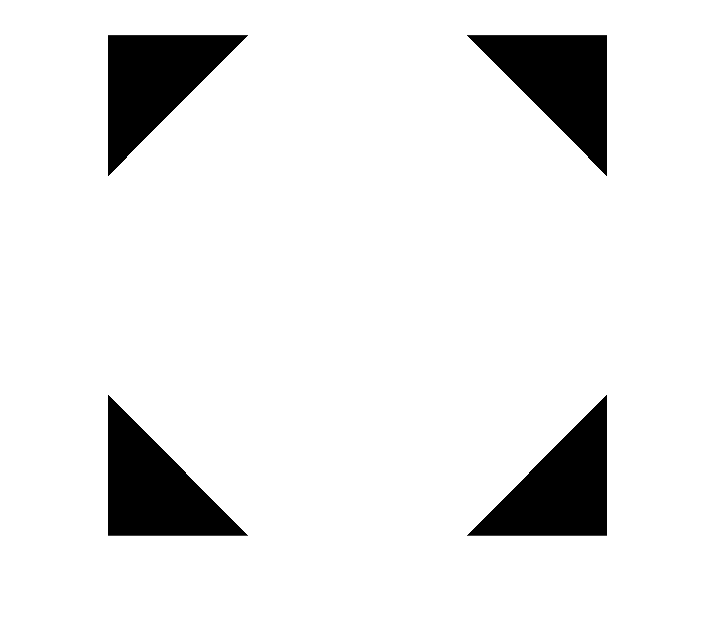
\includegraphics[width=0.7\linewidth]{strel.png}
    \caption{Example of a strel neighborhood.}
    \label{fig:strel}
\end{figure}
This \textit{strel} is moving over an image, when it covers an area with the same rgb value, the system knows it is in an area without a border.
But when the \textit{strel} is in an area that is covered with more than one different value, it is clear that their is a border present.
When there is a pixel of the \textit{strel} that has a lighter value \footnote{Lighter in greyscale value means a higher value} than the center pixel, the value of this center pixel becomes this lighter value.
When this is performed on an image, the lighter areas on the image will become bigger.
This is shown in figure~\vref{fig:dilate}.
\begin{figure}
    \centering
    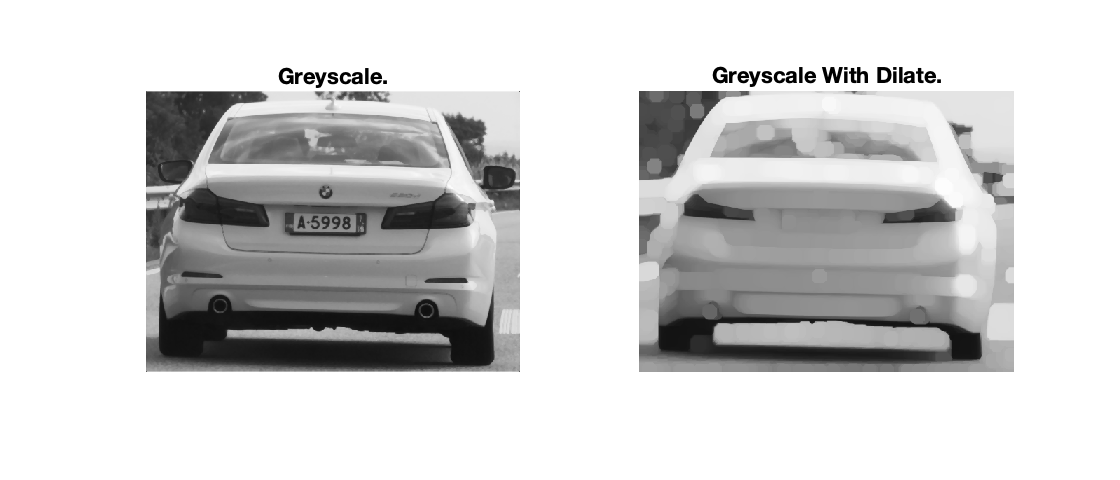
\includegraphics[width=0.9\linewidth]{dilate.png}
    \caption{Example of a dilated image.}
    \label{fig:dilate}
\end{figure}
\par
To successfully erode an image, it is necessary to have a neighborhood search area, this can be created using a \textit{strel} function.\cite{gonzalez2008digital}
Imagine to have a neighborhood that looks like a circle with radius of a few pixels. This is shown in figure~\vref{fig:strel}.
This \textit{strel} is moving over an image, when it covers an area with the same rgb value, the system knows it is in an area without a border.
But when the \textit{strel} is in an area that is covered with more than one different value, it is clear that their is a border present.\cite{gonzalez2008digital}
When there is a pixel of the \textit{strel} that has a darker value \footnote{Darker in greyscale value means a lower value} than the center pixel, the value of this center pixel becomes this darker value.
When this is performed on an image, the lighter areas on the image will become smaller.
This is shown in figure~\vref{fig:erode}.
\begin{figure}
    \centering
    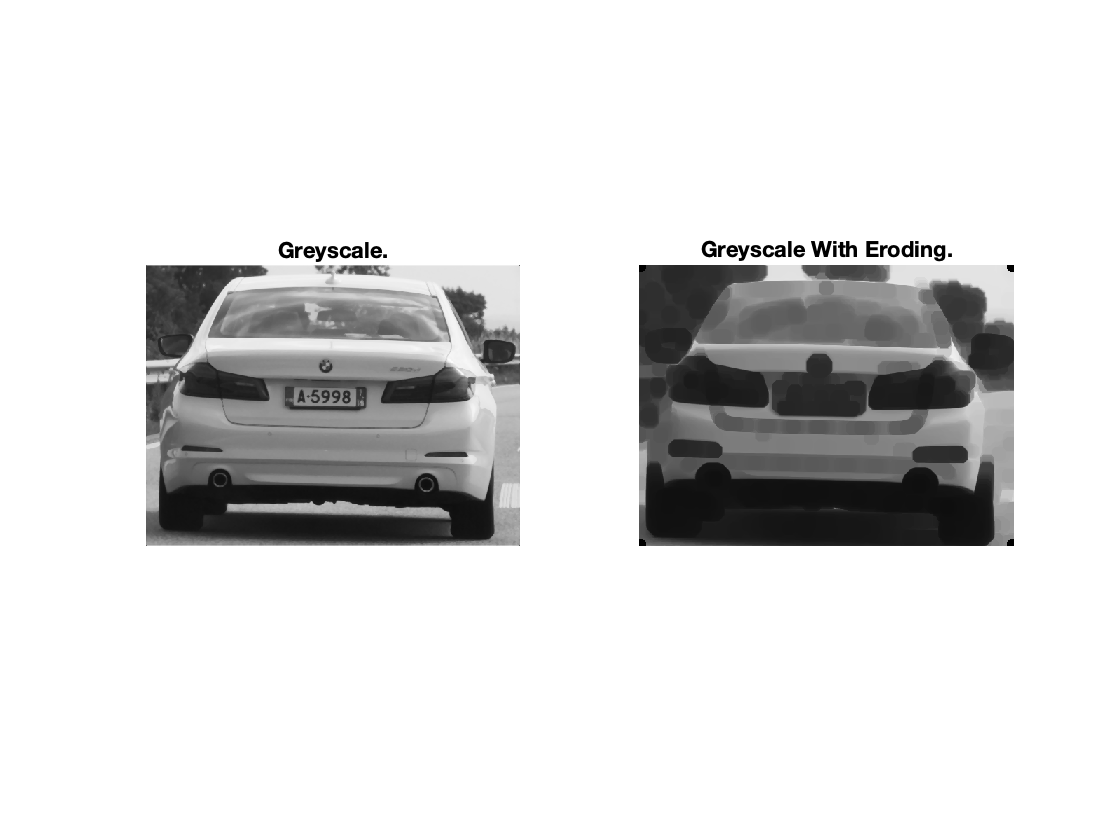
\includegraphics[width=0.9\linewidth]{erode.png}
    \caption{Example of a eroded image.}
    \label{fig:erode}
\end{figure}
\par
In the previous paragraphs, dilating and eroding is exaggerated.
When the radius of the \textit{strel} is reduced to 1, the edges can be exact determent when the the results are subtracted.
The result of this is shown in figure~\vref{fig:de}.
\begin{figure}
    \centering
    \includegraphics[width=0.9\linewidth]{DE.png}
    \caption{Example of an all edge detection}
    \label{fig:de}
\end{figure}
With this result we can conclude that sub problem~\vref{sub:detectAllEdges} is solved.
\par
With a quick recap we can recognize the fact that at this point we have an image with recognized edges.
However the goal of the image manipulation part is delivering interesting regions where to search for a license plate.
To get to that point there are two more necessary sub problems to solve: clear edges and delete non interesting edges, fill the interesting edges.
We start with clearing the image. 
The start point is an image as shown in figure~\vref{fig:de}.
To make a difference between the different kind of edges, it is necessary to em brighten the edges and completely en darken the rest of the picture.
This is possible by making the contrast bigger and than convert the image to a binary map.
By using a binary map, there are only two options: a border or no border, a 1 or a 0.
When converting the binary map back to a "normal" image we are now shore we have an image with only the borders/edges present.
The result at this point is an image with only clear edges, therefor it is safe to say that the objective of sub problem~\vref{sub:clearEdges} are achieved.

\subsubsection{Filling}
As stated in the previous paragraph, the objective of the image manipulation is the presentation of interesting regions.
What are interesting regions in the picture? Regions that possible contain a number or letter. 
A property of numbers and letters is that they mostly do not have a lot of straight lines. especially no single straight lines.
With this property in mind we can use another \textit{strel} function to remove straight lines. 
Instead of using a disk size strel, it is possible to use a linear strel, this will help detect the non interesting edges.
With the function \textit{imfill()}, it is possible to fill enclosed regions in the image. 
This is applied to the image, in theory, every enclosed region can be a letter or a number.
Non filled edges are thinned out with the result that the difference between them becomes bigger.
Results off these manipulations are shown in figure~\vref{fig:hf}.
These manipulations are combined with the earlier talked about linear edge removal.
An example of the final result after image manipulation is shown in figure~\vref{fig:finalim}.
\begin{figure}
    \centering
    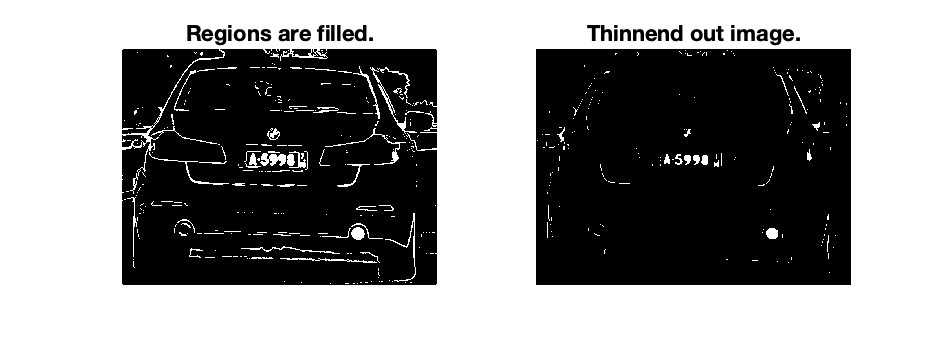
\includegraphics[width=0.8\linewidth]{hf.png}
    \caption{Example of region filling and thinning out the image.}
    \label{fig:hf}
\end{figure}
\begin{figure}
    \centering
    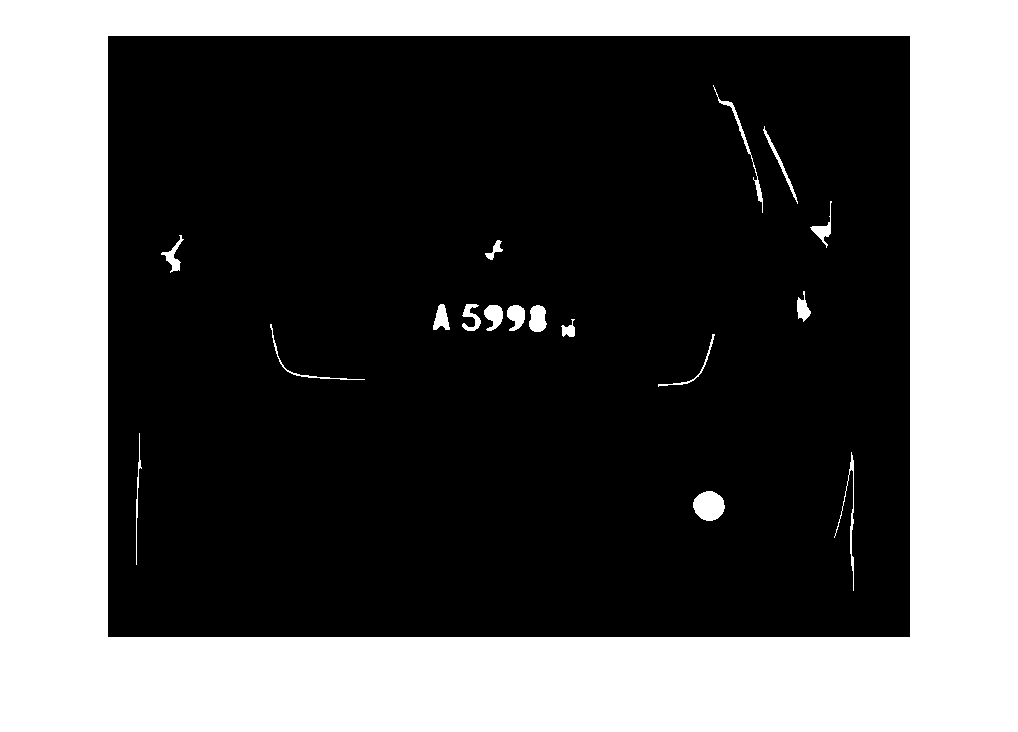
\includegraphics[width=0.8\linewidth]{finalim.png}
    \caption{Example of the final result after image manipulation.}
    \label{fig:finalim}
\end{figure}
Before starting with the search part, one addition is done to the image manipulation.
The function \textit{Iprops()} is called on the final result from the image manipulation.
This function produces containers over all the the different interesting parts in the pictures.
Two parts of this function are very interesting for the use in this case.
The tag 'Bounding Box', this produces practical information about the container in the form of four elements:
\begin{itemize}
    \item Starting X coordinate.
    \item Starting Y coordinate.
    \item Height.
    \item Width.
\end{itemize}
In that way are the complete dimensions of the container given.
The second tag is 'Image', this produces the image corresponding to the container dimensions.
Now all the elements are there to start the search operation.

\subsection{The Search}
The use of making a difference between image manipulation and the search is explained in the "Problem Breakdown" section.
In this subsection follows a detailed explanation of how the search works and how to adapt the search to different license plate layouts.

\subsubsection{Find Candidates}
The main objective is also the biggest question, how do start searching in the picture.
We know we have a picture with the regions selected but how can we confident say which regions to skip?
The answer to this question can partly be found in the knowledge we have about the containers.
We can assume the following: the containers corresponding to the different characters of the license plate will be in the same Y dimension.
So if it is possible to filter the containers on Y dimension it will be clear which regions are interesting and have possibly the license plate.
\par 
From the main script \textit{ReadLicensePlate.m}, listing~\vref{ReadLicensePlate}, the function \textit{findIndices} is called.
In this function, the sorting in regions start.
This is possible using the \textit{hist()} function, with parameter the Y starting point of the different containers.
The hist function makes a histogram, standard dividing the complete range into 10 parts.
This function uses a BucketSort mechanism.\footnote{BucketSort is a fast but not so precise sorting algorithm.}
After executing this function it is possible to see how much containers there are in every region.
Because the specifics of the license plate are given in the main script, it is justified to say that all regions with less containers than total license plate characters are not interesting.
In this way we only keep the regions with a lot of containers.
\par
Only filtering on Y coordinate is not enough.
It is safer to make a safety mechanism with another factor.
By multiplying the Y coordinate with the width of the container we get a new factor to filter.
This second factor is used as a backup when the first filter is unable to give use full results.
\par
After the filtering, all the regions with at least as many items as there have to be characters in the license plate, are selected.
Every region is looked into.
The histogram corresponding to the example used in the image manipulation can be found in figure~\vref{fig:hist}.
The next major challenge is that regions can have more containers than that there are characters.
A selection procedure is necessary to select which of these containers are not part of the license plate.
This selection is done in the function \textit{eliminateOptions}.
The function gets the selection of containers as input as well as the images corresponding to these containers, the amount of characters in a license plate and the amount of letters in a license plate.
This function is run in a for-loop on every interesting region.
\begin{figure}
    \centering
    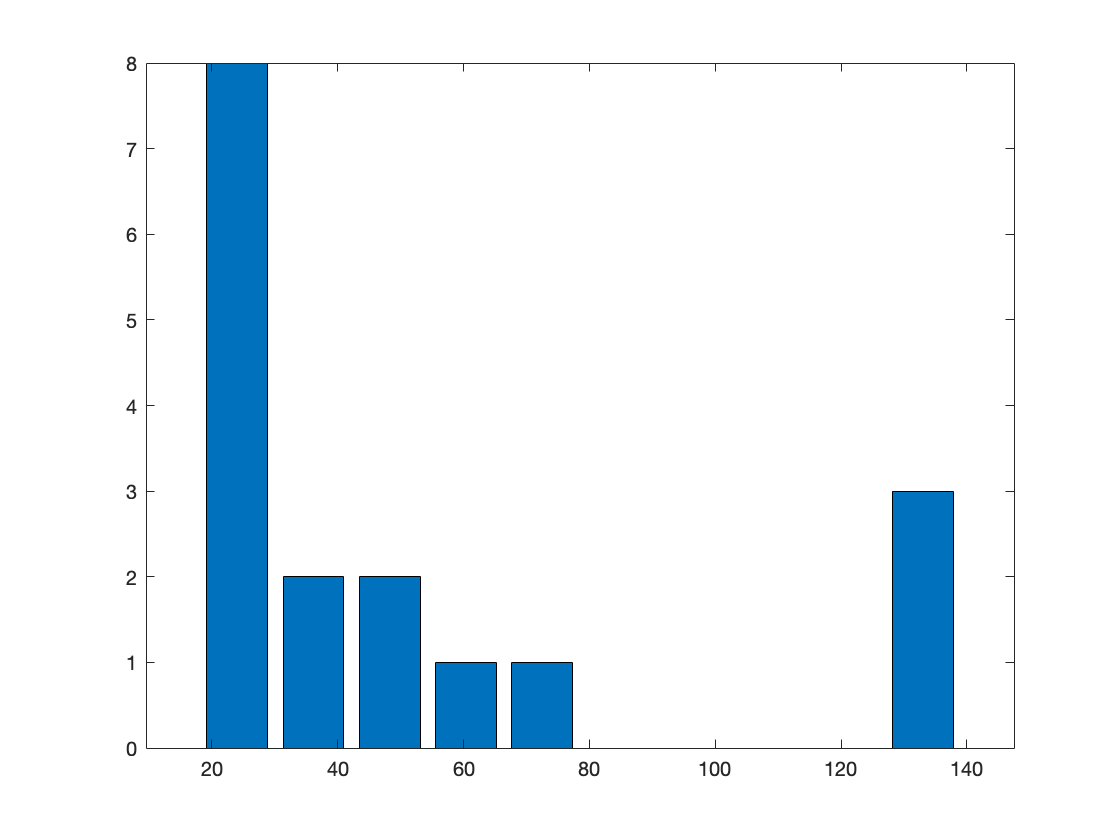
\includegraphics[width=0.6\linewidth]{hist.png}
    \caption{Histogram corresponding to the picture used in the image manipulation example.}
    \label{fig:hist}
\end{figure}

\subsubsection{Testing}
The testing happens in the function \textit{eliminateOptions}, can be found in listing~\vref{eliminateOptions}.
All containers in the region are matched to a character, by the function \textit{readLetter}.
This function not only returns the letter that is matched to the corresponding container but also the correlation factor.
This correlation factor is very important because after the matching, the filtering has to start.
The filtering of the containers is done in a while loop and continuous as long as there are more characters left than that there are in a license plate.
In every iteration of the while loop will the character with the lowest correlation be tracked down and deleted.
In this way it is safe to say that the best option for this region will come out of this function.

\subsubsection{Choice}
This sub problem is solved in the function \textit{ReadLicensePlate}.
After the for-loop done on all possible regions, we have a possible license plate for every interesting region.
Except for the license plate, the function \textit{findIndices} also returned an average correlation factor for the complete license plate.
This average factor is used to select the license plate with the highest possibility.
At this point the system returns the license plate found in the original picture and this is therefor the end of the system.
The system returns the license plate in ASCII code, what means that these are not the character values but this is easier if the Matlab scripts are ever going to be used in another software program.
Also most languages support an easy conversion from ASCII code to character value.


